\documentclass[pdftex,10pt,a4paper,oneside]{report}

\usepackage{amsmath}
\usepackage{amssymb} 
% \usepackage{algorithm}
% \usepackage{algorithmic}
\usepackage{svg}
\usepackage{fancyhdr}
\usepackage{graphicx}
\usepackage{lipsum}
\usepackage{multirow}
\usepackage{setspace}
\usepackage{verbatim}
\usepackage{booktabs}
\usepackage{tabularx}
\usepackage{caption}
\usepackage{subcaption}
\usepackage{array}
\usepackage[linesnumbered,ruled,vlined]{algorithm2e}
\usepackage{float}
\usepackage{pbox}

\usepackage[
    hidelinks,
    colorlinks=true,
    linkcolor=black,    % 章节链接颜色
    citecolor=blue,     % 引用颜色
    urlcolor=blue       % URL 颜色
]{hyperref}

\fancyhf{}
\pagestyle{fancy}
\renewcommand{\headrulewidth}{0.2pt}
\renewcommand{\bibname}{References}

% Styles can be Sonny, Lenny, Glenn, Conny, Rejne, Bjarne and Bjornstrup
\usepackage[Sonny]{fncychap}

\begin{document}

% !TEX root =  ../Dissertation.tex

\thispagestyle{empty}

\begin{spacing}{2}
	\begin{center}
		
\includegraphics[scale = 1.5]{Preamble/BirmCrest.png}
	\end{center}
	\vspace{10mm}
	\begin{center}
		\textbf{\Large The Project Title}
		\vspace{10mm}
	\end{center}
	\begin{center}
		\textbf{\large The Document Title}
		\vspace{20mm}
		\\\textbf{\Large Matthew Leeke}
		\vspace{30mm}
	\end{center}
	\begin{center}
		{\large School of Computer Science}
		\\ {\large College of Engineering and Physical Sciences}
		\\ {\large University of Birmingham}
		\\ {\large 2023-24}
	\end{center}
\end{spacing}

\pagenumbering{roman}



\chapter*{Abstract}
\addcontentsline{toc}{chapter}{Abstract}

The 0/1 Knapsack Problem (KP) is a canonical NP-complete combinatorial optimization challenge with wide-ranging applications.
While traditional exact algorithms like Dynamic Programming are computationally infeasible for large-scale instances due to exponential time or memory complexity, \
 recent deep learning approaches often struggle with generalization to problem sizes unseen during training.
This paper addresses this scalability challenge by proposing a novel, end-to-end reinforcement learning (RL) framework designed for high-performance generalization.

We present a solution based on the Proximal Policy Optimization (PPO) algorithm, employing a sophisticated model architecture that \
features a shared Transformer encoder to capture the global, combinatorial relationships between items, an actor head with a Pointer Network-based decoder for item selection, \
 and a separate Multi-Layer Perceptron (MLP) critic head for stable value estimation.
This entire workflow is encapsulated in a reusable Python package, which handles data generation, preprocessing, model training, and comparative evaluation against various benchmarks.

Trained exclusively on small-scale KP instances with 5 to 50 items, our model demonstrates powerful generalization capabilities.
When tested on large-scale instances of up to 200 items, the framework achieves a stable Mean Relative Error (MRE) below 30\% against optimal solutions derived from the Gurobi solver.
Experimental results confirm that our approach significantly outperforms baseline neural architectures, including pure MLPs and earlier Pointer Network models, \
 in terms of solution quality and exhibits greater training stability than the REINFORCE algorithm.
This work validates the effectiveness of a PPO-based framework for solving combinatorial optimization problems, \
 presenting a robust and scalable method that bridges the gap between traditional solvers and modern neural networks.

\vspace{1em}
% \begin{quotation}
\noindent\small\textbf{Keywords:} 0/1 Knapsack Problem, Reinforcement Learning, Proximal Policy Optimization (PPO), Generalization, Transformer, Pointer Network
% \end{quotation}
% % !TEX root =  ../Dissertation.tex

\thispagestyle{empty}
\addcontentsline{toc}{chapter}{Dedication}

\begin{center}
	Dedicated to...
\end{center}

\newpage
 % Comment out for UG dissertations

\chapter*{Acknowledgements}
\addcontentsline{toc}{chapter}{Acknowledgements}

I would first and foremost like to express my deepest gratitude to my supervisor Prof. Li and inspector Prof. Jiao, for their invaluable guidance and unwavering support throughout this research journey. Their profound expertise and insightful feedback were instrumental in shaping the direction of this project and my development as a researcher.

I am also incredibly grateful to my friends, for the stimulating discussions, collaborative spirit, and the invaluable suggestions they offered regarding this project. The academic community we shared was a constant source of motivation and inspiration.

My heartfelt thanks go to my family. Their unconditional love, endless encouragement, and profound patience have been the bedrock of my academic pursuits. This accomplishment would not have been possible without their unwavering support.

Finally, I wish to acknowledge the unique era in which this research was conducted. The advent of advanced AI has fundamentally enhanced my ability to explore and has made it easier than ever to transform ideas into reality. It feels as though AI is a great equalizer, lifting the baseline of knowledge and capability for all. I am profoundly grateful to be conducting research in what I believe is the most exciting time in history.
% !TEX root =  ../Dissertation.tex

\chapter*{Declarations}
\addcontentsline{toc}{chapter}{Declarations}
 % Comment out for UG dissertations
% % !TEX root =  ../Dissertation.tex

\chapter*{Sponsorship and Grants}
\addcontentsline{toc}{chapter}{Sponsorship and Grants}

The research presented in this dissertation was made possible by the support of the following benefactors and sources:

\begin{itemize}

\item The Department of Computer Science, University of Warwick, Coventry, United Kingdom - Some Award (2004-2012)


\end{itemize} % Comment out for UG dissertations

\chapter*{Abbreviations}
\addcontentsline{toc}{chapter}{Abbreviations}

\begin{flushleft}

ACB \hfill  Apple Banana Carrot

\end{flushleft}
%% !TEX root =  ../Dissertation.tex

\chapter*{Notations}
\addcontentsline{toc}{chapter}{Notations}

\begin{flushleft}

{\bf $r_2$} \hfill  Has some meaning

\end{flushleft}
 % Comment out for most dissertations 
% !TEX root =  ../Dissertation.tex

\tableofcontents


% !TEX root =  ../Dissertation.tex

\listoffigures
\addcontentsline{toc}{chapter}{List of Figures}

\listoftables
\addcontentsline{toc}{chapter}{List of Tables}

\newpage

% !TEX root =  ../Dissertation.tex

\pagenumbering{arabic}

\renewcommand{\chaptermark}[1]{\markboth{#1}{}}
\rhead{\small \thechapter . \leftmark}
\lfoot{\centering \thepage}



% \chapter{Introduction}
% !TEX root =  ../Dissertation.tex

\chapter{Introduction}

% overview of this chapter

% !TEX root = ../Dissertation.tex
\section{Research Overview}

This dissertation documents the development of an end-to-end reinforcement learning (RL) framework for solving the 0/1 Knapsack Problem (KP) with a primary focus on scalability and generalization. The research journey commenced with an empirical validation of classical optimization algorithms. Initial experiments with methods such as Dynamic Programming and Branch and Bound confirmed their well-documented theoretical limitations; they proved to be computationally infeasible for problems with large capacity constraints or a high number of items, suffering from excessive memory usage and exponential runtime complexity respectively.

Following this, the investigation transitioned to machine learning paradigms. A preliminary exploration using a standard Multi-Layer Perceptron (MLP) architecture quickly revealed its inability to learn a generalizable solving policy, as evidenced by its poor performance on unseen problem sizes. To overcome the limitations of supervised learning, which relies on the availability of high-quality, optimal solution labels, this research pivoted towards reinforcement learning. The theoretical foundation for this shift is the inherent connection between dynamic programming and RL, as the DP recurrence for the Knapsack Problem can be viewed as a deterministic instance of the Bellman equation \cite{tamarValueIterationNetworks2017}.

The initial RL approach was inspired by the seminal work of Bello et al. \cite{belloNeuralCombinatorialOptimization2017}, which utilized a Pointer Network with the REINFORCE algorithm. However, our replication and experimentation with this method highlighted significant training instability and high variance, which are common challenges associated with vanilla policy gradient methods. To address these shortcomings, this work proposes a substantially evolved framework. The final architecture employs a shared Transformer encoder to effectively capture the combinatorial inter-dependencies of the items, a Pointer Network-based decoder as the actor, and an MLP critic head. The training is stabilized and made more efficient by leveraging the Proximal Policy Optimization (PPO) algorithm \cite{schulmanProximalPolicyOptimization2017}. This novel framework successfully learns a scalable policy, achieving a solution accuracy of approximately 70\% (equivalent to a Mean Relative Error below 30\%) on large-scale generalization tests.
% !TEX root = ../Dissertation.tex
\section{Motivation}

The 0/1 Knapsack Problem (KP) is a canonical problem in the field of combinatorial optimization and computer science, formally classified as NP-complete \cite{cappartCombinatorialOptimizationReasoning2022}. Its importance is twofold. Theoretically, as many NP-complete problems are reducible to one another, advancements in solving the KP can provide insights applicable to a wide range of other computationally hard problems. Practically, the KP serves as a mathematical abstraction for numerous real-world decision-making scenarios, including portfolio optimization, resource allocation, and logistics planning.

Despite its significance, the development of scalable and generalizable solvers remains a major challenge. Traditional exact algorithms, while guaranteeing optimality, are not viable for large-scale instances that are common in industrial applications. This has motivated a growing interest in machine learning-based approaches \cite{wangSolvingCombinatorialOptimization2024}. However, a review of recent literature reveals a critical research gap: the majority of existing neural network-based solvers are designed and trained for specific, fixed problem sizes \cite{belloNeuralCombinatorialOptimization2017}. These models often fail to generalize their learned policies to instances with a different number of items than they were trained on, severely limiting their practical utility.

Furthermore, within the sub-field of deep reinforcement learning for combinatorial optimization, the fundamental 0/1 Knapsack Problem has received surprisingly little attention compared to other problems like the Traveling Salesperson Problem. The lack of a truly end-to-end framework that can be trained on smaller instances and effectively generalize to larger, unseen ones represents a significant and compelling opportunity for research. This dissertation is motivated by the goal of addressing this gap by developing a novel RL framework that learns a robust and scalable policy for the 0/1 Knapsack Problem.
% !TEX root = ../Dissertation.tex
\section{Contributions}

This dissertation presents a series of contributions to the field of applying deep reinforcement learning to combinatorial optimization problems. The primary contributions are summarized as follows:

\begin{itemize}
    \item \textbf{A Novel, Generalizable RL Framework for the 0/1 Knapsack Problem:} We propose and validate an end-to-end deep reinforcement learning framework built upon the Proximal Policy Optimization (PPO) algorithm \cite{schulmanProximalPolicyOptimization2017}. The architecture's core, a shared Transformer encoder \cite{koolAttentionLearnSolve2019a} paired with a Pointer Network decoder \cite{belloNeuralCombinatorialOptimization2017} and an MLP critic, is specifically designed to learn the underlying structure of the KP, enabling it to scale effectively.

    \item \textbf{Empirical Demonstration of Scalable Generalization:} A key contribution is the rigorous empirical evidence that our model learns a genuine, scalable solving policy rather than merely memorizing solutions for fixed-size problems. Trained exclusively on small-scale instances (5 to 50 items), the model demonstrates strong generalization to large, unseen instances (up to 200 items), maintaining a stable and low Mean Relative Error below 30\% when compared to the optimal solutions provided by the Gurobi solver. This capability marks a significant advancement over prior neural approaches that were limited to fixed problem dimensions.

    \item \textbf{A Comprehensive and Reproducible Software Platform:} The entire framework has been implemented as a robust and reusable Python package. By leveraging well-regarded libraries such as Gymnasium and Stable Baselines 3, this work provides a comprehensive platform for the entire research pipeline, including procedural data generation, model training, and the comparative evaluation of RL agents against both traditional algorithms and commercial solvers. This platform serves as a valuable tool for ensuring reproducibility and fostering further research in the domain.
\end{itemize}

% ..

% \chapter{Related Work}
% !TEX root = ../Dissertation.tex
\chapter{Related Work}
\label{chap:related_work}

While traditional algorithms such as Dynamic Programming provide the theoretical foundation for solving Combinatorial Optimization Problems (COPs), contemporary research has predominantly shifted towards Machine Learning (ML) methodologies to overcome their scalability limitations.
Within the last decade, and especially in the last few years, Reinforcement Learning (RL) has emerged as the dominant paradigm for training agents to solve these problems, owing to its ability to learn effective heuristics through direct interaction with a problem environment.
Following the effective taxonomy proposed in the survey by Wang et al. \cite{wangSolvingCombinatorialOptimization2024}, this chapter reviews the state-of-the-art by categorizing these DNN-based approaches into two main families: \textit{constructive} and \textit{improvement} methods.

\section{Constructive Methods}
Constructive methods build a solution from scratch, typically in a sequential, element-by-element manner.
This paradigm is largely dominated by encoder-decoder architectures that learn to output a sequence or a set of items that form the final solution.
In the context of the Knapsack Problem, researchers have explored various RL-based constructive methods. For instance, \textbf{Yildiz (2022)} compared the performance of fully connected, attention, and Transformer models within a Deep Q-Network (DQN) framework \cite{yildizReinforcementLearningUsing2022}. \textbf{Afshar et al. (2020)} introduced a state aggregation approach to mitigate the state-space explosion and combined it with the A2C algorithm \cite{afsharStateAggregationApproach2020}. Others have extended these methods to more complex variants like the Multi-Knapsack Problem (MKP) \cite{surDeepReinforcementLearningBased2022}.

\subsection{Vanilla Pointer Networks}
The initial application of neural networks to constructive solutions was marked by the Pointer Network (Ptr-Net), first proposed by Vinyals et al. to be trained with Supervised Learning (SL) on solution labels from existing solvers \cite{vinyalsPointerNetworks2017}.
However, the reliance on expensive-to-generate optimal labels was a significant bottleneck. A major breakthrough came from \textbf{Bello et al. (2017)} \cite{belloNeuralCombinatorialOptimization2017}, who successfully trained a Ptr-Net using the REINFORCE algorithm with a critic baseline.
This pivotal work demonstrated that an agent could learn to solve both the Traveling Salesman Problem (TSP) and the Knapsack Problem effectively without supervised data.
Following this, \textbf{Nazari et al. (2018)} extended this RL-based Ptr-Net approach to handle problems with dynamic elements, such as the Capacitated Vehicle Routing Problem (CVRP) \cite{nazariReinforcementLearningSolving2018}.

\subsection{Pointer Networks with Self-Attention}
A crucial architectural evolution was the replacement of Recurrent Neural Network (RNN) based encoders with the Transformer architecture, which uses self-attention mechanisms to better capture the global context of the entire problem instance at once.
Deudon et al. were among the first to apply this to COPs. A highly influential paper by \textbf{Kool et al. (2019)} \cite{koolAttentionLearnSolve2019a} solidified this trend with their "Attention Model". They paired a Transformer encoder with a more efficient "rollout baseline" for the REINFORCE algorithm, achieving state-of-the-art results on TSP and CVRP and setting a new benchmark for subsequent research.

\subsection{Hierarchical Pointer Networks}
To tackle large-scale COPs or those with complex constraints, researchers have developed hierarchical frameworks.
These methods typically decompose a large problem into smaller, manageable subproblems, which are then solved by a neural model.
For instance, Ma et al. presented a Graph Pointer Network within a hierarchical RL architecture to address TSP with time windows.
Similarly, other works like Pan et al. have successfully applied hierarchical models to solve large-scale TSP (LSTSP), demonstrating a promising direction for scaling neural COP solvers \cite{wangSolvingCombinatorialOptimization2024}.

\section{Improvement Methods}
In contrast to constructive methods, improvement methods begin with a complete (often randomly or greedily generated) solution and iteratively refine it.
This is typically achieved by learning a policy that guides a local search or other heuristic optimization process.

\subsection{Local Search Based on Neural Networks}
This class of methods trains a neural network to act as a sophisticated operator within a local search framework.
The network learns to identify which parts of a current solution are most promising to modify.
Chen and Tian developed the "NeuRewriter" framework, where a Ptr-Net trained with an Actor-Critic algorithm learns to select both a rewrite rule and a region of the solution to apply it to, showing strong results on Job Shop Scheduling (JSP) and CVRP.
More recently, architectures have shifted towards Transformers. For example, Ma et al. proposed the Dual-Aspect Collaborative Transformer (DACT) and used \textbf{PPO} to train a policy that improves CVRP solutions iteratively \cite{wangSolvingCombinatorialOptimization2024}.

\subsection{Heuristics Assisted by Neural Networks}
Another effective improvement strategy is to use a DNN to enhance a critical component of a powerful traditional heuristic.
The Lin-Kernighan-Helsgaun (LKH) algorithm is one of the most effective traditional heuristics for the TSP. Recognizing this, Xin et al. proposed NeuroLKH, which uses a Graph Convolutional Network (GCN) to predict a promising set of candidate edges.
This learned knowledge is then used to guide and prune the search space of the LKH algorithm, achieving remarkable performance by combining the strengths of both deep learning and classical heuristics \cite{wangSolvingCombinatorialOptimization2024}. Beyond assisting traditional heuristics, researchers have also explored hybrid approaches, such as combining RL with scatter search \cite{zhaoReinforcementLearningdrivenCooperative2024} or with Constraint Programming (CP) to leverage their respective strengths \cite{cappartCombiningReinforcementLearning2021}.

\section{The Rise of Proximal Policy Optimization}
The training stability of early policy gradient methods like REINFORCE was a significant challenge, as they are known to suffer from high variance in gradient estimates, leading to inefficient learning.
A landmark development in this area was the introduction of the Proximal Policy Optimization (PPO) algorithm by \textbf{Schulman et al. (2017)} \cite{schulmanProximalPolicyOptimization2017}. PPO stabilizes the training process by optimizing a "clipped surrogate objective" function, which discourages the policy from changing too drastically in a single update.
This provides the reliability of more complex trust-region methods but with a much simpler implementation, striking a favorable balance between sample complexity, simplicity, and performance.
Due to its robustness, PPO has become a go-to algorithm in the RL community and has been successfully applied to COPs.
For example, \textbf{Gholipour et al. (2023)} \cite{gholipourTPTOTransformerPPOBased2023} leveraged a Transformer-PPO architecture to effectively solve the task offloading problem in edge computing. Similarly, \textbf{Que et al. (2023)} also successfully combined a Transformer with PPO to tackle the 3D Packing Problem, further demonstrating the power of this algorithmic combination \cite{queSolving3DPacking2023}.

\section{Positioning the Present Work}
This dissertation situates itself within the modern, end-to-end constructive paradigm while leveraging state-of-the-art advancements in RL algorithms.
The proposed framework is built upon the following foundations:
\begin{itemize}
    \item It follows the \textbf{constructive, reinforcement learning} approach pioneered by Bello et al. \cite{belloNeuralCombinatorialOptimization2017}, learning a policy from scratch without reliance on supervised labels.
    \item It adopts a \textbf{Transformer-based encoder}, in line with the current state-of-the-art for capturing complex, non-sequential relationships in combinatorial problems, following the success of models like that of Kool et al. \cite{koolAttentionLearnSolve2019a}.
    \item It employs the \textbf{Proximal Policy Optimization (PPO)} algorithm for its proven training stability and high performance, as established by Schulman et al. \cite{schulmanProximalPolicyOptimization2017}.
\end{itemize}

While many advanced DRL applications have focused on routing problems like TSP and CVRP, this work applies the powerful Transformer-PPO architecture specifically to the 0-1 Knapsack Problem with a strong emphasis on \textbf{generalization} from small to large-scale instances.
This addresses a critical gap, as many prior works were confined to fixed problem sizes \cite{belloNeuralCombinatorialOptimization2017}.
Recent related studies, such as that by \textbf{Zhang et al. (2025)} \cite{zhangReinforcementLearningSolving2025}, have also tackled the KP with RL but have explored different avenues, such as value-based Dueling DQN combined with state representation normalization and Noisy layers for exploration.
Our focus on a state-of-the-art policy gradient method contributes a valuable perspective to the ongoing effort to develop scalable and generalizable solvers for this fundamental combinatorial optimization problem.

\begin{table}[H]
    \centering
    \caption{Summary of Key Related Works in Learning-based COPs}
    \label{tab:related_work_summary}
    \small
    \begin{tabular}{@{}lllll@{}}
        \toprule
        \textbf{Work} & \textbf{Model / Architecture} & \textbf{Method} & \textbf{Generalization} \\
        \midrule
        Bello et al. \cite{belloNeuralCombinatorialOptimization2017} & Ptr-Net + RNN & REINFORCE & To fixed size\\
        Kool et al. \cite{koolAttentionLearnSolve2019a} & Transformer & REINFORCE& Improved but focused \\
        Gholipour et al. \cite{gholipourTPTOTransformerPPOBased2023} & Transformer & PPO & Problem-specific \\
        Zhang et al. \cite{zhangReinforcementLearningSolving2025} & Transformer & Dueling DQN & To fixed size \\
        \midrule
        \textbf{This Work} & 
        \begin{tabular}[c]{@{}c@{}}{Transformer +} \\ {Ptr-Net Decoder}\end{tabular} & 
        \begin{tabular}[c]{@{}c@{}}{RL (PPO)} \\ {+ MLP Critic}\end{tabular} & 
        \begin{tabular}[c]{@{}c@{}}{End-to-end} \\ {+ Generalization}\end{tabular} &  \\
        \bottomrule
    \end{tabular}
\end{table}

% \chapter{Background}
% !TEX root =  ../Dissertation.tex

\chapter{Background}

% !TEX root = ../Dissertation.tex
\section{What is the 0/1 Knapsack Problem?}

The Knapsack Problem (KP) is a quintessential problem in combinatorial optimization, serving as a fundamental model for resource allocation under constraints. It is formally classified as an NP-complete problem, meaning there is no known algorithm that can find the optimal solution in polynomial time for all instances. This work focuses on the most common and classic variant: the 0/1 Knapsack Problem.

\subsection{Problem Definition}

In the 0/1 Knapsack Problem, one is given a set of items, each with an associated weight and value, and a knapsack with a fixed capacity. The objective is to select a subset of these items to place into the knapsack such that the total value of the selected items is maximized, without exceeding the knapsack's weight capacity.

The "0/1" property is a crucial constraint: for each item, the decision is binary. The item can either be fully included in the knapsack (represented by 1) or completely excluded (represented by 0). It is not possible to include a fraction of an item.

\subsection{Mathematical Formulation}

The problem can be formulated formally as follows. Let there be \(n\) items. For each item \(i \in \{1, 2, \dots, n\}\), let:
\begin{itemize}
    \item \(v_i > 0\) be its value,
    \item \(w_i > 0\) be its weight.
\end{itemize}
Let \(W\) be the maximum capacity of the knapsack.

We define a binary decision variable \(x_i\) for each item \(i\):
\[
x_i = 
\begin{cases} 
1 & \text{if item } i \text{ is selected,} \\
0 & \text{if item } i \text{ is not selected.} 
\end{cases}
\]

The goal is to choose the values for \(x_1, x_2, \dots, x_n\) in order to solve the following integer linear programming problem:

\begin{equation}
\label{eq:objective}
\text{maximize} \quad Z = \sum_{i=1}^{n} v_i x_i
\end{equation}

\begin{equation}
\label{eq:constraint}
\text{subject to} \quad \sum_{i=1}^{n} w_i x_i \leq W
\end{equation}

\begin{equation}
\label{eq:binary}
\text{with} \quad x_i \in \{0, 1\} \quad \forall i \in \{1, 2, \dots, n\}
\end{equation}

Here, Equation~\ref{eq:objective} represents the objective function, which is the total value of the items selected. Equation~\ref{eq:constraint} is the capacity constraint, ensuring that the total weight of the selected items does not surpass the knapsack's limit. Finally, Equation~\ref{eq:binary} enforces the binary nature of the decision for each item.
% !TEX root = ../Dissertation.tex
\section{What is Dynamic Programming?}
\label{sec:dp}

Dynamic Programming (DP) is a classical method for solving complex optimization problems by breaking them down into simpler, overlapping subproblems. As an exact algorithm, DP guarantees finding the optimal solution. For the 0/1 Knapsack Problem, DP is not only a cornerstone of traditional computer science but also provides the theoretical bedrock for virtually all modern reinforcement learning approaches. The core principle connecting them is the Bellman equation, which is fundamental to both methodologies.

DP can be implemented in two primary ways:

\begin{itemize}
    \item \textbf{Tabulation (Bottom-up):} This approach systematically solves every subproblem, starting from the smallest ones, and stores the results in a table (or a multi-dimensional array). It then builds upon these stored results to solve larger and more complex subproblems until the final solution is reached. This method is exhaustive as it computes the value for every possible state.

    \item \textbf{Memoization (Top-down):} This approach is a recursive method that solves the main problem by breaking it down. However, it stores the result of each computed subproblem in a lookup table. Before computing a subproblem, it first checks if the result is already stored. If it is, the stored result is reused; otherwise, the subproblem is computed and its result is stored for future use. This way, it only computes the states that are actually reached during the recursive calls.
\end{itemize}

\subsection{The State-Transition Equation}

For the 0/1 Knapsack Problem, the DP approach relies on defining a state and a value function. Let \(V(i, w)\) be the maximum value that can be obtained using a subset of the first \(i\) items with a knapsack capacity of \(w\). The state-transition equation, or DP recurrence, is defined as follows:

\begin{equation}
\label{eq:dp_recurrence}
V(i, w) = 
\begin{cases} 
V(i-1, w) & \text{if } w_i > w \\
\max(V(i-1, w), v_i + V(i-1, w - w_i)) & \text{if } w_i \leq w 
\end{cases}
\end{equation}

The first case corresponds to the decision of not including item \(i\) (as it exceeds the current capacity \(w\)), so the optimal value is the same as the one obtained with \(i-1\) items. The second case represents the core decision: we take the maximum of either excluding item \(i\) (the value remains \(V(i-1, w)\)) or including it (the value is \(v_i\) plus the optimal value achievable with \(i-1\) items and the remaining capacity \(w - w_i\)).

This recurrence is directly analogous to the Bellman equation, which is central to reinforcement learning:
\begin{equation}
\label{eq:bellman}
V^{\pi}(s) = \mathbb{E}_{\pi} [R_{t+1} + \gamma V^{\pi}(S_{t+1}) | S_t = s]
\end{equation}

The principles are identical: the value of a state is determined by the immediate reward plus the value of the subsequent state(s). In the context of a deterministic, model-based problem like the Knapsack Problem, the DP recurrence (Equation~\ref{eq:dp_recurrence}) is an exact, specific instance of the Bellman equation (Equation~\ref{eq:bellman}). The key distinction is that the Bellman equation provides a more general framework that can be extended to model-free scenarios where the state-transition probabilities are unknown and must be learned.

\subsection{Complexity and Limitations}

Despite its optimality, the standard DP approach for the knapsack problem has significant drawbacks that limit its applicability to large-scale instances:

\begin{itemize}
    \item \textbf{High Complexity:} Both the tabulation and memoization methods suffer from high computational complexity. The time and space complexity are both \(O(nW)\), where \(n\) is the number of items and \(W\) is the knapsack capacity. This leads to slow execution times and the risk of memory explosion when \(W\) is exponentially large relative to the input size.
    
    \item \textbf{Pseudo-Polynomial Time:} The \(O(nW)\) complexity is considered pseudo-polynomial because the runtime depends on the numeric value of the input \(W\), not just the size of the input (i.e., the number of bits required to represent \(W\)). When \(W\) grows exponentially with respect to its bit-length (e.g., \(W=2^n\)), the runtime becomes exponential in the input size---a hallmark of NP-hard problems.
\end{itemize}

\subsection{Optimizations and Their Inadequacies}

Several optimizations have been developed to mitigate these issues, but they do not fully resolve the scalability problem for large instances.

\begin{itemize}
    \item \textbf{Space Optimization:} The space complexity of the tabulation method can be optimized from \(O(nW)\) to \(O(W)\) by noticing that the calculation for row \(i\) only depends on the results from row \(i-1\). This can be achieved by using a one-dimensional array. However, this optimization comes at the cost of losing the ability to reconstruct the optimal item set without additional bookkeeping, as intermediate results are overwritten. Furthermore, the time complexity remains \(O(nW)\), which is still prohibitive.

    \item \textbf{Fully Polynomial-Time Approximation Scheme (FPTAS):} For the 0/1 Knapsack Problem, an FPTAS exists, which guarantees a solution with a value of at least \((1-\epsilon)\) times the optimal value. It works not by normalizing capacity, but by scaling and rounding the item \textit{values}. Given a desired approximation ratio \(\epsilon > 0\), the algorithm proceeds by setting a scaling factor \(K = (\epsilon v_{\max}) / n\), where \(v_{\max} = \max_{i} v_i\). Each item's value is then transformed to \(v'_i = \lfloor v_i / K \rfloor\). A standard DP algorithm is then run on these scaled, integer values. The time complexity of this approach is \(O(n^3/\epsilon)\), which is polynomial in both \(n\) and \(1/\epsilon\). Despite this, for the large-scale problems with many items addressed in this research, the computational cost can still be unacceptable.
\end{itemize}

\begin{table}[htbp]
    \centering
    \caption{Theoretical Complexity of Traditional Algorithms}
    \label{tab:complexity_comparison}
    \small
    \begin{tabular}{@{}l l l p{5cm}@{}}
        \toprule
        \textbf{Algorithm} & \textbf{TC} & \textbf{SC} & \textbf{Notes} \\
        \midrule
        DP & $O(nC)$ & $O(C)$ & Exact. Pseudo-polynomial time complexity. \\
        BnB & $O(2^n)$ & $O(n)$ & Exact. Exponential in the worst-case. \\
        Greedy & $O(n \log n)$ & $O(n)$ & Approximation. Fast but suboptimal. \\
        FPTAS & $O(n^3/\epsilon)$ & $O(n^2/\epsilon)$ & Approximation. Polynomial in $n$ and $1/\epsilon$. \\
        \bottomrule
    \end{tabular}

    % Using a minipage to format the note below the table
    \begin{minipage}{0.9\textwidth}
        \vspace{2pt} % Adds a small space between the table and the note
        \small % Use \small for the note, which is more readable than \tiny
        \textbf{Note:} TC: Time Complexity, SC: Space Complexity. $n$: number of items, $C$: knapsack capacity, $\epsilon$: approximation ratio.
    \end{minipage}
\end{table}
% !TEX root = ../Dissertation.tex
\section{Basics of Reinforcement Learning}
\label{sec:rl}

Given the inherent limitations of both exact algorithms and traditional heuristics for solving large-scale combinatorial optimization problems, this research turns to Reinforcement Learning (RL) as a promising alternative paradigm.

\subsection{Why Reinforcement Learning?}

The motivation for employing RL is best understood by comparing it to other dominant approaches for solving complex problems: supervised learning, commercial solvers, and metaheuristics.

\begin{itemize}
    \item \textbf{In Comparison to Supervised Learning (SL):} The primary advantage of RL is its independence from large datasets of high-quality, labeled solutions. For a problem like the 0/1 Knapsack, generating such labels would require running a commercial exact solver (e.g., Gurobi). This presents a paradox: if a commercial solver can efficiently find the optimal solution to generate a label, the problem for that specific instance is already solved, rendering the training of an SL model for that purpose somewhat redundant. RL circumvents this by learning directly from interaction and a scalar reward signal. However, it is worth noting that SL can be synergistically combined with RL, for instance, by using imitation learning to pre-train an agent from expert (solver-generated) demonstrations to accelerate the learning process.

    \item \textbf{In Comparison to Commercial Solvers:} While solvers like Gurobi or CPLEX are powerful tools that guarantee optimality, their runtime often scales exponentially with problem size for NP-hard problems. For very large or complex instances, finding the optimal solution can become computationally intractable. Furthermore, they typically operate as deterministic "black boxes," offering less flexibility in stochastic or dynamic environments. In contrast, a trained RL agent learns a \textit{policy}---a mapping from states to actions---that can generate high-quality solutions very quickly (often in constant or near-constant time) once trained, making it highly suitable for applications requiring rapid decision-making.

    \item \textbf{In Comparison to Metaheuristics:} Algorithms like Genetic Algorithms (GA) or Simulated Annealing (SA) provide another alternative. However, their performance is highly sensitive to a set of hyperparameters that require extensive, problem-specific tuning. Crucially, these parameters often need to be re-tuned when the scale or characteristics of the problem instances change. Moreover, they can be prone to premature convergence to local optima. An RL model, once successfully trained, encapsulates a generalized solving strategy. It can be invoked directly to solve any problem instance within the distribution it was trained on, up to a specified maximum scale, without the need for re-tuning for each new instance.
\end{itemize}

\subsection{What is Reinforcement Learning?}

Reinforcement Learning is a paradigm of machine learning where an \textit{agent} learns to make a sequence of optimal decisions by interacting with an \textit{environment}. The agent's goal is to learn a policy that maximizes a cumulative reward signal over time. This interaction is typically modeled as a Markov Decision Process (MDP).

The core of RL is the agent-environment interaction loop, as depicted in Figure~\ref{fig:ae_loop}. At each timestep \(t\), the agent observes the environment's state \(S_t\) and, based on its policy, selects an action \(A_t\). The environment transitions to a new state \(S_{t+1}\) and provides the agent with a scalar reward \(R_{t+1}\) as feedback on its action. This process repeats, allowing the agent to learn from the consequences of its actions.

\begin{figure}[htbp]
    \centering
    % Note: Ensure the path is correct relative to your main .tex file
    % If Dissertation.tex is in '.../dissertation/', this path should work.
    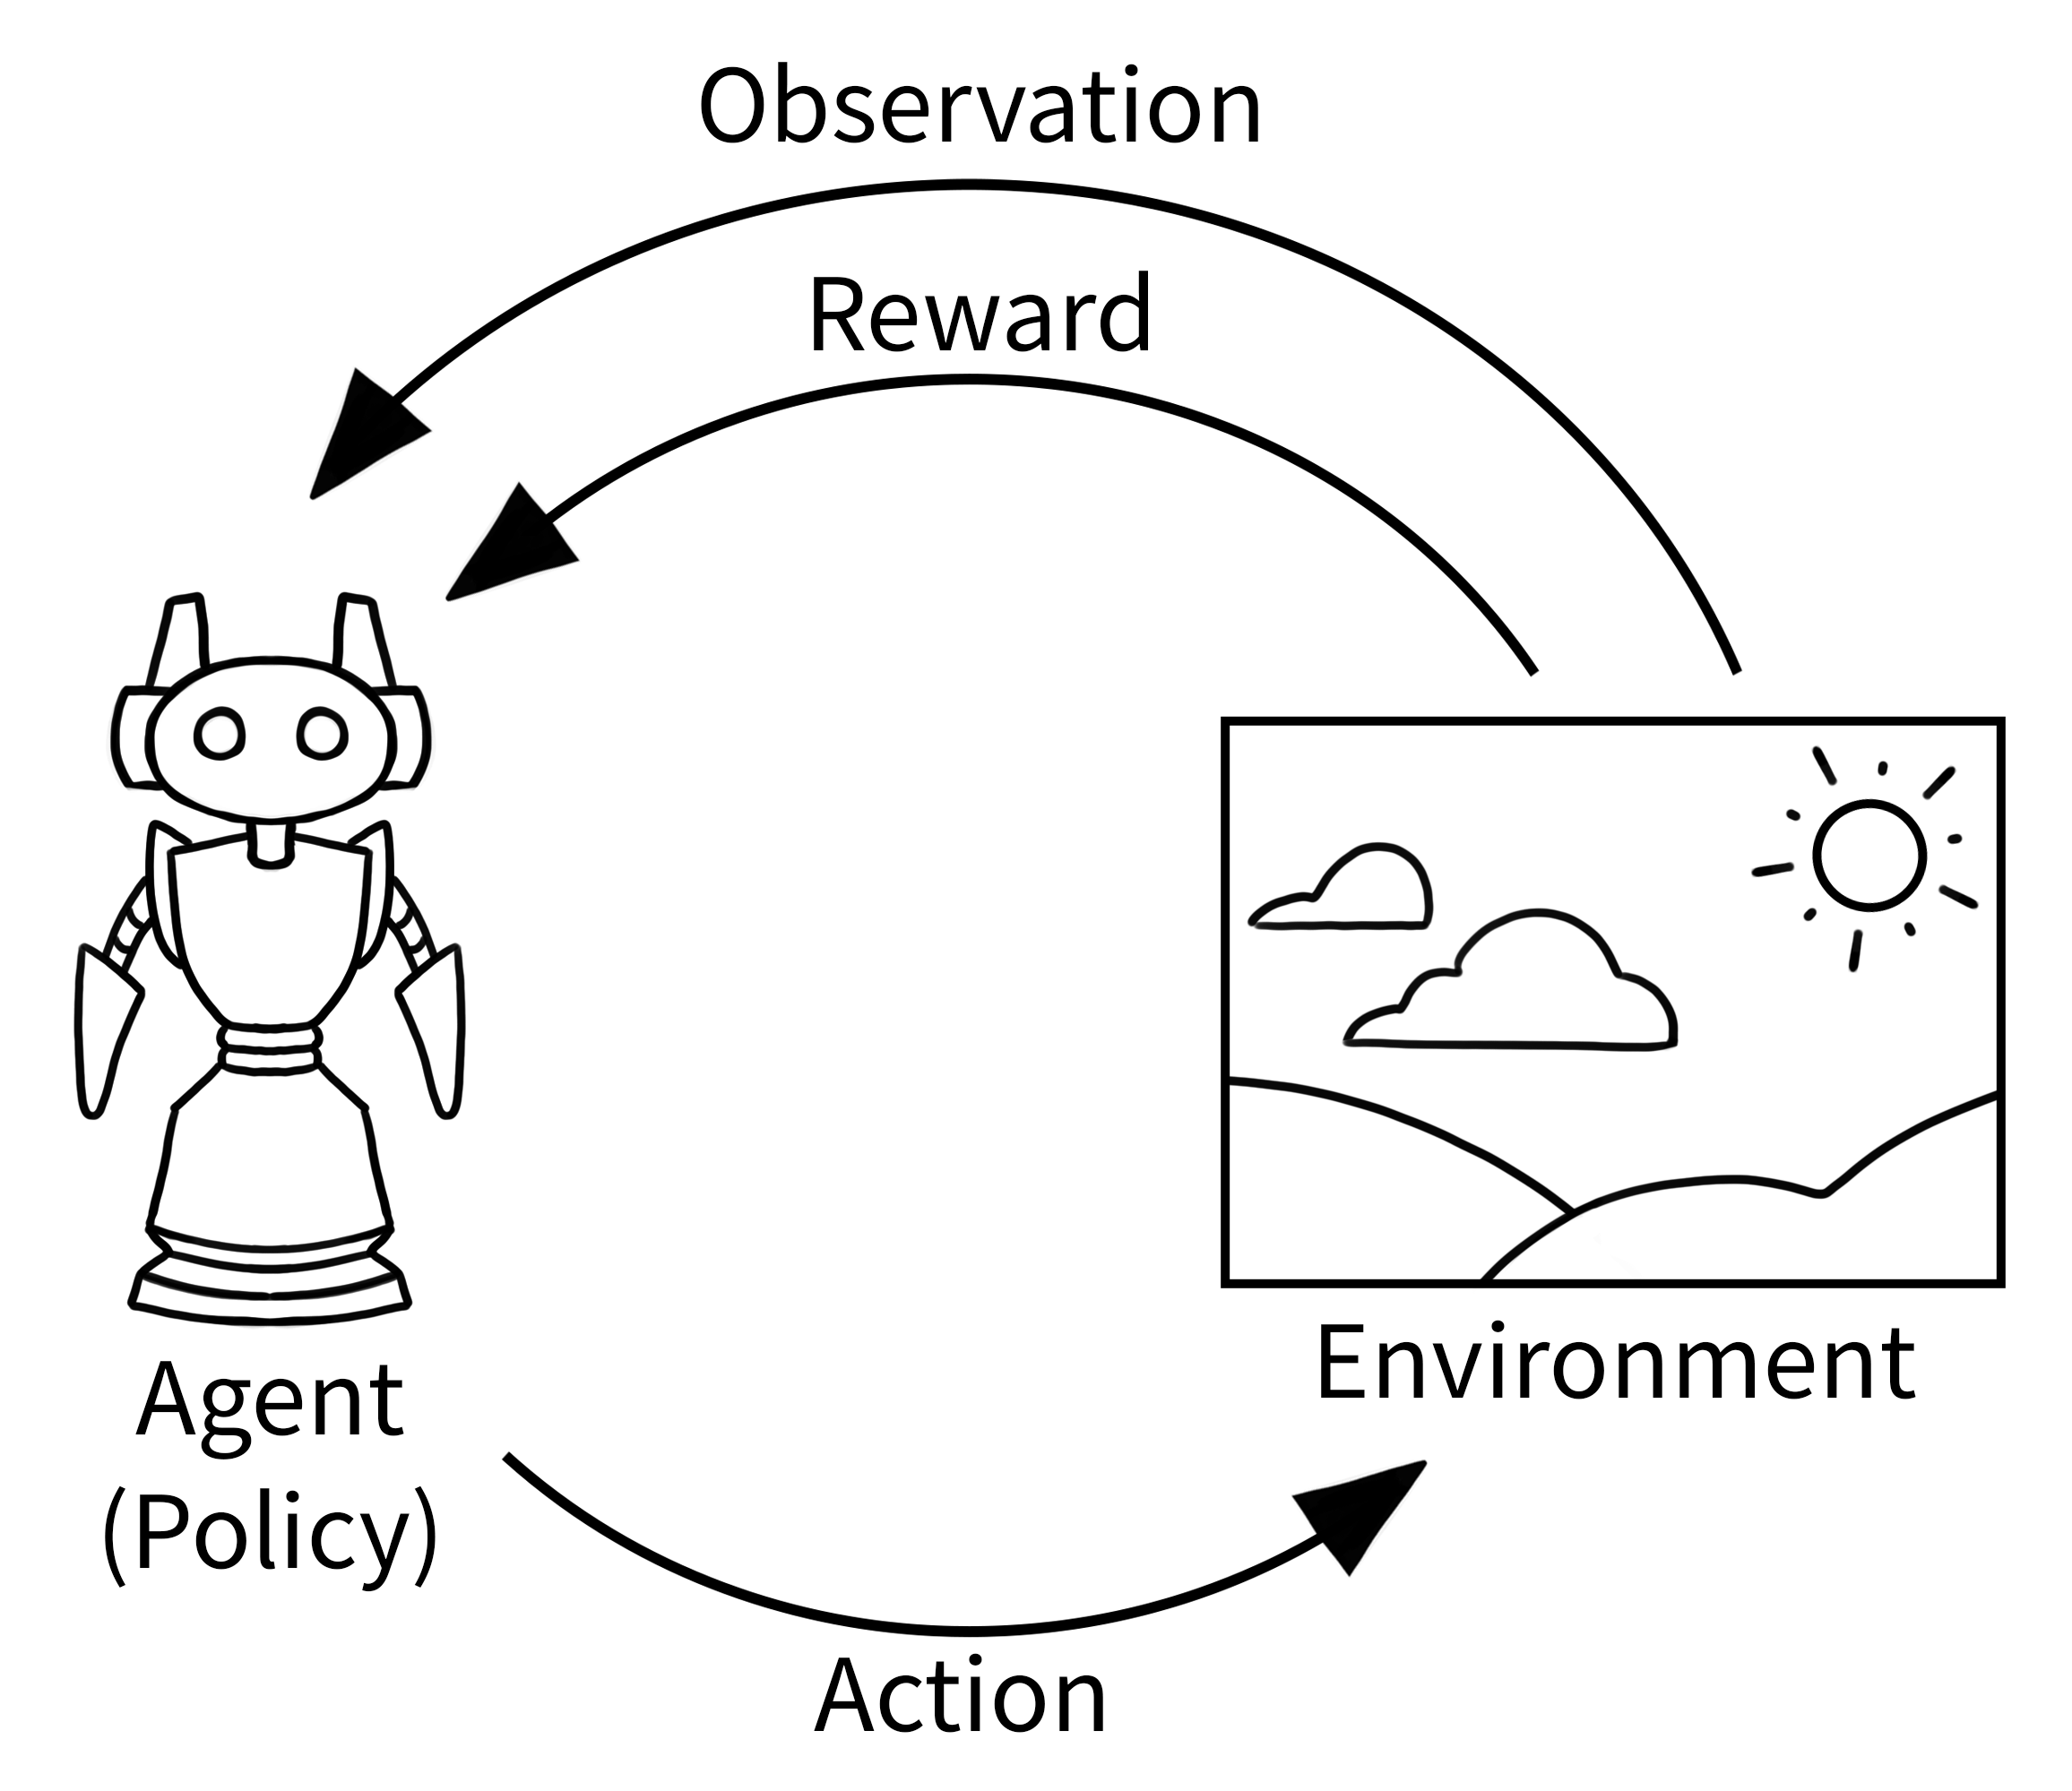
\includegraphics[width=0.8\textwidth]{figures/AE_loop.png}
    \caption{The standard agent-environment interaction loop in Reinforcement Learning. Source: Gymnasium Documentation.}
    \label{fig:ae_loop}
\end{figure}

A critical distinction from other machine learning paradigms is the nature of the training data. The agent does not learn from a static dataset of raw problem data (e.g., item weights and values). Instead, the learning process is driven by data generated dynamically through interaction. This data takes the form of trajectories or experiences, which are sequences of tuples:
\[ (S_t, A_t, R_{t+1}, S_{t+1}) \]
By collecting these experiences, the agent refines its policy to favor actions that lead to higher long-term cumulative rewards. For the Knapsack Problem, this means learning a sequence of item selections that ultimately yields the highest total value without violating the capacity constraint.
% !TEX root = ../Dissertation.tex
\subsection{From Bellman to PPO: An Evolutionary Trajectory}
\label{sec:from-bellman-to-ppo}

The transition from Dynamic Programming (DP) to modern reinforcement learning algorithms like Proximal Policy Optimization (PPO) is not arbitrary. It follows a coherent, problem-driven evolution rooted in the Bellman equation. This evolution can be understood as a sequence of adaptations, each designed to overcome a critical limitation of the previous approach to achieve the scalability, efficiency, and stability required for complex problems like the 0/1 Knapsack Problem.

\subsubsection{The Foundational Bellman Equation}
As established in Section~\ref{sec:dp}, the DP recurrence is a specific instance of the Bellman principle. The general, element-wise Bellman equation for the state-value function \(V^\pi(s)\) is:
\begin{equation}
    \label{eq:bellman_elementwise}
    V_{\pi}(s) = \sum_{a \in A} \pi(a|s) \left[ \sum_{r \in R} p(r|s, a)r + \gamma \sum_{s' \in S} p(s'|s, a)V_{\pi}(s') \right]
\end{equation}
Here, the terms are defined as:
\begin{itemize}
    \item \(\pi(a|s)\) is the \textbf{policy}, defining the probability of taking action \(a\) in state \(s\).
    \item \(p(s'|s, a)\) and \(p(r|s, a)\) together form the \textbf{model} of the environment, specifying the probabilities of transitioning to state \(s'\) and receiving reward \(r\), respectively.
    \item \(\gamma\) is the \textbf{discount factor} (\(0 \le \gamma \le 1\)), which balances immediate and future rewards. Although the Knapsack Problem is theoretically an undiscounted, finite-horizon problem, our framework adopts \(\gamma = 0.99\). This choice aligns with standard practice in deep reinforcement learning, where a discount factor close to 1 is often used to stabilize training and reduce the variance of value estimates. The state transitions in the KP environment are also deterministic constants.\end{itemize}
DP is a \textbf{model-based} approach because it requires full knowledge of the model (the transition and reward probabilities) to compute the value function. In contrast, most RL applications are \textbf{model-free}, learning a policy through trial-and-error without explicit knowledge of the environment's dynamics.

\subsubsection{Step 1: Bellman to Value Function Approximation}
\textbf{Limitation of DP:} A tabular representation of \(V(s)\) is intractable for large-scale problems due to exponential memory and computational requirements.

\textbf{Adaptation:} Replace the exact, tabular value function with a \textit{learnable function approximator} \(V_\phi(s)\), typically a neural network with parameters \(\phi\). This allows generalization across states and enables application to high-dimensional state spaces.
\[
V^\pi(s) \quad \longrightarrow \quad V_\phi(s) \approx V^\pi(s)
\]

\subsubsection{Step 2: Value Approximation to Policy Gradient}
\textbf{Limitation of Value-Based Methods:} Methods like DQN, which learn a value function and derive a policy indirectly (e.g., \(\pi(s) = \arg\max_a Q(s,a)\)), are ill-suited for the Knapsack Problem. The action space (the set of available items) is large, discrete, and dynamically changes at each step. Iterating through all possible actions to find the `argmax` is inefficient and does not scale. A more effective approach is to directly learn a stochastic policy that outputs a probability distribution over the available items.

\textbf{Adaptation:} Directly parameterize the policy as \(\pi_\theta(a|s)\) and optimize its parameters \(\theta\) to maximize the expected return. This transition involves several layers of approximation:
\begin{enumerate}
    \item \textbf{Function Approximation:} The policy \(\pi\) is approximated by a neural network \(\pi_\theta\).
    \item \textbf{Sampling Approximation:} The expectation \(\mathbb{E}_{\tau \sim \pi_\theta}[\cdot]\) over all possible trajectories is approximated by averaging over a finite batch of trajectories sampled from the current policy.
    \item \textbf{Policy Gradient Theorem:} This provides a theoretical tool to compute the gradient of the expected return, enabling optimization via gradient ascent.
\end{enumerate}
The REINFORCE algorithm implements this via the policy gradient, using a Monte Carlo estimate of the expected return.

\subsubsection{Step 3: Monte Carlo Estimation to Actor-Critic (TD)}
\textbf{Limitation of Monte Carlo Estimation:} The REINFORCE algorithm uses the full cumulative return \(G_t = \sum_{k=t}^{T} \gamma^{k-t} R_{k+1}\) to update the policy. This Monte Carlo estimator, while unbiased, suffers from high variance because the return for an action at timestep \(t\) is affected by all subsequent rewards and stochastic decisions. This results in noisy gradient estimates and unstable learning.

\textbf{Adaptation:} Replace the MC estimator with a lower-variance Temporal Difference (TD) estimator. TD learning updates an estimate based on an observed reward and another learned estimate (a process called bootstrapping). The TD error, \(\delta_t = R_{t+1} + \gamma V_\phi(s_{t+1}) - V_\phi(s_t)\), provides a less noisy, step-by-step learning signal. In the Actor-Critic framework, this principle is used to compute the \textit{advantage function}, \(\hat{A}_t\), which measures how much better an action is than the average expectation from that state.
\[
G_t \quad \longrightarrow \quad \hat{A}_t = R_{t+1} + \gamma V_\phi(s_{t+1}) - V_\phi(s_t)
\]
Using \(\hat{A}_t\) as the credit assignment signal in the policy gradient update reduces variance and enables more efficient and stable online learning.

\subsubsection{Step 4: Actor-Critic to Proximal Policy Optimization (PPO)}
\textbf{Limitation of standard Actor-Critic:} Unconstrained policy updates can still lead to catastrophic performance drops. A single bad mini-batch could result in an overly large gradient step, moving the policy to a poor region of the parameter space from which it cannot easily recover.

\textbf{Adaptation:} PPO \cite{schulmanProximalPolicyOptimization2017} introduces a \textit{clipped surrogate objective} that limits the magnitude of policy change at each update, effectively creating a trust region.
\[
\mathcal{L}^{\text{CLIP}}(\theta) = \mathbb{E}_{t} \left[ \min\left( r_t(\theta) \hat{A}_t, \text{clip}(r_t(\theta), 1-\epsilon, 1+\epsilon) \hat{A}_t \right) \right]
\]
where the probability ratio \(r_t(\theta) = \frac{\pi_\theta(a_t|s_t)}{\pi_{\theta_{\text{old}}}(a_t|s_t)}\) measures the policy change. The clipping mechanism prevents \(r_t(\theta)\) from deviating too far from 1, thereby penalizing large policy updates. This simple but effective stabilization allows PPO to achieve robust, high-performance learning, making it the algorithm of choice for this research.

\subsubsection{Summary of the Evolutionary Path}
The entire trajectory, driven by the need to address specific limitations at each stage, is summarized in Table~\ref{tab:evolution_path}.

\begin{table}[htbp]
    \centering
    \small
    \caption{Evolutionary Path from Dynamic Programming to PPO}
    \label{tab:evolution_path}
    \begin{tabularx}{\textwidth}{l >{\raggedright\arraybackslash}X}
        \toprule
        \textbf{Stage} & \textbf{Key Change from Previous Stage} \\
        \midrule
        \textbf{1. DP} & 
        (Baseline) Solves problems using a complete, exact state-value table. \\

        \textbf{2. Value-Based RL} & 
        Replaces the exact table with a neural network (\textit{function approximator}) to handle large state spaces. \\

        \textbf{3. Policy Gradient} & 
        Directly parameterizes and optimizes the policy network, instead of learning values to infer a policy. \\

        \textbf{4. Actor-Critic / PPO} & 
        Uses a TD-based advantage estimate to replace high-variance Monte Carlo returns, and adds a clipping mechanism to stabilize training. \\
        \bottomrule
    \end{tabularx}
\end{table}

% \chapter{Methodology}
% !TEX root = ../Dissertation.tex
\chapter{Methodology}
\label{chap:methodology}

This chapter details the methodology developed to solve the 0/1 Knapsack Problem (KP) using a scalable, end-to-end deep reinforcement learning framework.
We begin by reformulating the combinatorial optimization problem as a sequential decision process suitable for RL.
Subsequently, we describe the overall reinforcement learning framework, justify the selection of the Proximal Policy Optimization (PPO) algorithm, and present our novel neural network architecture.
Finally, we elaborate on the critical mechanisms of reward design and action masking that ensure solution feasibility, and conclude with the specifics of our training strategy and implementation to ensure reproducibility.

\section{Problem Formulation as a Sequential Decision Process}
The first critical step in applying reinforcement learning is to reframe the KP from a static combinatorial optimization problem into a sequential decision-making task.
To this end, we formally model the problem as a finite-horizon, discounted Markov Decision Process (MDP) with a discount factor $\gamma = 0.99$.
An agent interacts with a KP environment over a sequence of discrete timesteps, selecting one item at a time to place into the knapsack.
The components of the MDP are defined as follows:
\begin{itemize}
    \item \textbf{State (\(s_t\))}: The state at timestep \(t\) provides a complete snapshot of the current problem-solving status. It is a dictionary containing all necessary information for the agent to make a decision. The state space \(S\) is defined by the tuple \(s_t = \{ \mathbf{I}, C_t, \mathbf{m}_t \}\), where:
    \begin{itemize}
        \item \(\mathbf{I} \in \mathbb{R}^{N_{max} \times 2}\) is a tensor representing the features of all items (normalized weight and value), padded to a maximum length \(N_{max}\).
        \item \(C_t \in \mathbb{R}^+\) is a scalar representing the remaining capacity of the knapsack at timestep \(t\).
        \item \(\mathbf{m}_t \in \{0, 1\}^{N_{max}}\) is a binary mask vector indicating which actions (items) are currently valid.
    \end{itemize}
    \item \textbf{Action (\(a_t\))}: An action \(a_t\) corresponds to the selection of a single item \(i\) from the set of currently available items.
    This selection is determined by the policy network, which, in our case, is implemented as a Pointer Network that outputs a probability distribution over the items.
    \item \textbf{Action Space (\(A_t\))}: The action space is dynamic and state-dependent.
    At any given state \(s_t\), the set of valid actions consists of all items \(i\) that have not yet been selected and whose weight \(w_i\) does not exceed the remaining capacity \(C_t\).
    This dynamic control over the action space is enforced through the action mask \(\mathbf{m}_t\).
    \item \textbf{Reward (\(r_t\))}: To guide the agent's learning process, we employ a dense reward scheme.
    When the agent selects a valid item \(i\), it receives an immediate reward equal to that item's value, \(r_t = v_i\).
    This provides a direct and immediate signal about the quality of each incremental decision.
    \item \textbf{Episode Termination}: An episode concludes when no more items can be placed into the knapsack, i.e., when the action mask \(\mathbf{m}_t\) becomes a zero vector. This occurs either because all items have been considered or because the weight of every remaining item exceeds the current capacity.
\end{itemize}
By structuring the KP in this autoregressive manner, we transform it into a constrained combinatorial search process that is exceptionally well-suited for being solved by a neural agent that learns a sequential decoding policy.

\section{Reinforcement Learning Framework}
Our framework is built upon two widely adopted, high-quality open-source libraries: \texttt{Gymnasium} and \texttt{Stable-Baselines3}. \texttt{Gymnasium}, a fork of OpenAI's original Gym library, provides a standardized API for defining and interacting with reinforcement learning environments. By conforming to this API, our custom `KnapsackEnv` becomes compatible with a vast ecosystem of RL algorithms.

For the algorithm implementation, we use \texttt{Stable-Baselines3}, a library that provides robust, well-tested, and state-of-the-art implementations of deep RL algorithms. The choice of Proximal Policy Optimization (PPO)~\cite{schulmanProximalPolicyOptimization2017} from this library is deliberate. PPO is an on-policy, actor-critic algorithm renowned for its stability and sample efficiency. Its signature feature is a clipped surrogate objective function, which prevents excessively large policy updates and maintains a trust region around the current policy. This mechanism ensures more stable and reliable training convergence, a crucial factor when dealing with complex policy landscapes like those in combinatorial optimization. This stability was empirically validated in our preliminary experiments, where PPO consistently converged to high-quality policies.

\section{Neural Architecture Design}
The core of our proposed method is a novel neural architecture designed to effectively capture the complex, non-sequential relationships inherent in the Knapsack Problem. The model follows an encoder-decoder structure with a shared encoder and two distinct heads for the actor and the critic, as depicted in Figure~\ref{fig:model_architecture}.

\begin{figure}[H]
    \centering
    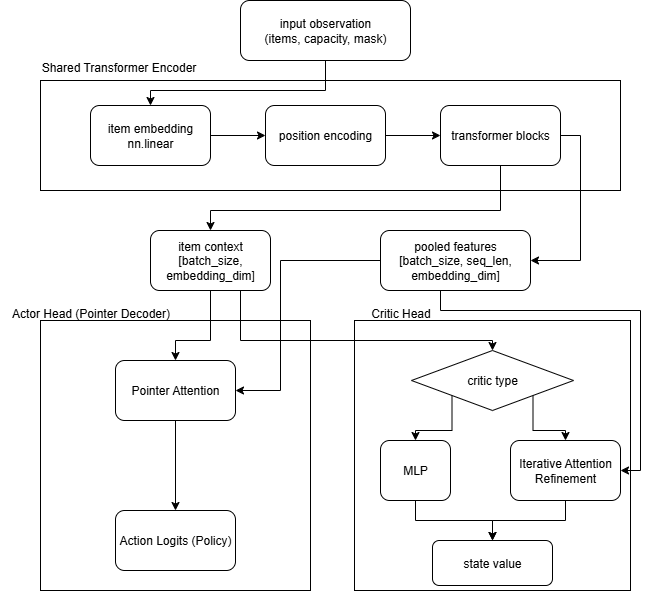
\includegraphics[width=0.9\textwidth]{figures/ppo_model_manual.png}
    \caption{The proposed neural architecture. An input observation is processed by a shared Transformer encoder to produce item-specific contexts and a global pooled feature vector. These are then consumed by a Pointer Network-based actor head and an MLP-based critic head.}
    \label{fig:model_architecture}
\end{figure}

\subsection{Shared Transformer Encoder}
The encoder's role is to process the raw problem instance and generate context-aware embeddings for each item. The input for each item \(i\) is its normalized weight \(w_i\) and value \(v_i\). We employ a \textbf{Transformer encoder} rather than a sequential model like an RNN. Its multi-head self-attention mechanism allows the model to weigh the importance of all other items when encoding a specific item, thereby capturing the global combinatorial structure of the problem. This is critical for the KP, where the decision to include one item is heavily dependent on the properties of all other available items. The encoder outputs two key tensors: a set of rich, context-aware embeddings for each item, \(\mathbf{H}_{context} \in \mathbb{R}^{B \times N_{max} \times D}\), and a global problem embedding, \(\mathbf{h}_{pooled} \in \mathbb{R}^{B \times D}\), derived by mean-pooling the item embeddings.

\subsection{Actor Head: Pointer Network-based Decoder}
The actor head, which implements the policy \(\pi_\theta(a|s)\), is a \textbf{Pointer Network}~\cite{vinyalsPointerNetworks2015}. This architecture is perfectly suited for our selection task as it directly outputs a probability distribution over the input items, rather than predicting a class from a fixed-size vocabulary. This avoids the limitation of a standard MLP, which would struggle to handle variable numbers of items and lacks the mechanism to directly reference inputs. At the same time, it is more efficient than a full Transformer decoder, as it does not need to generate new embeddings, only to point to existing ones.

Our implementation, the `PointerDecoder`, operates autoregressively. At each decoding step, it uses an attention mechanism to decide which item to select next. Its operation can be broken down as follows:
\begin{enumerate}
    \item \textbf{Initial Query}: At the first step, the decoder's initial query vector is the global problem embedding \(\mathbf{h}_{\text{pooled}}\) from the encoder.
    \item \textbf{Glimpse Mechanism}: To refine this query, we employ a "glimpse" mechanism, as implemented in \texttt{custom\_policy.py}. The query is used to attend over all item embeddings in \(\mathbf{H}_{\text{context}}\). A weighted sum of the context vectors, based on the attention scores, creates a new, more refined query vector. This process is repeated for a fixed number of iterations (\texttt{n\_glimpses=2}), allowing the model to iteratively focus its attention.
    \item \textbf{Additive Attention}: The attention scores are calculated using an additive attention mechanism. Both the item context vectors and the current query vector are projected into a common space. Their sum is passed through a \(\tanh\) activation, and the final score is computed via a dot product with a learnable parameter vector \(\mathbf{v}\). The logits \(u_i\) for item \(i\) are computed as:
    \[ u_i = \mathbf{v}^T \tanh(\mathbf{W}_c \mathbf{h}_i + \mathbf{W}_q \mathbf{q}) \]
    where \(\mathbf{h}_i\) is the context embedding for item \(i\), \(\mathbf{q}\) is the current query vector, and \(\mathbf{W}_c, \mathbf{W}_q, \mathbf{v}\) are learnable parameters.
    \item \textbf{Output}: After the final glimpse, the refined query is used one last time to compute the final attention scores (logits) over all items. These logits, after applying the action mask, are passed through a softmax function to produce the final probability distribution \(\pi_\theta(a_t|s_t)\).
    \item \textbf{Autoregressive Update}: For subsequent steps in the decoding sequence, the query is updated to be the embedding of the item that was just selected in the previous step, informing the next decision.
\end{enumerate}

\subsection{Critic Head: MLP for Value Estimation}
Based on our most successful experimental results (`Exp26`), the critic head is a simple yet effective Multi-Layer Perceptron (MLP) that estimates the state-value function \(V_\phi(s)\). This contrasts with more complex attention-based critics, which we found did not yield superior performance for this problem.

The critic's architecture is intentionally straightforward. Its sole input is the \textbf{global problem embedding}, \(\mathbf{h}_{pooled}\), which is the mean-pooled output of the shared Transformer encoder. This vector serves as a condensed representation of the entire state. The MLP then processes this vector through several linear layers with ReLU activations, LayerNorm, and Dropout to produce a single scalar value. This scalar represents the critic's estimate of the expected discounted cumulative reward (the value) from the current state.

By sharing the powerful Transformer encoder, the critic benefits from the same rich feature representation as the actor. However, using a simple MLP head for the value function, which is independent of the more complex actor head, improves training stability and efficiency.

\section{Training Techniques}
To ensure the reproducibility and robustness of our results, we employed several key training techniques and followed a standardized procedure.
\begin{itemize}
    \item \textbf{Input Pre-processing}: Before an instance is fed to the agent, a crucial pre-processing step is applied: the items are sorted in descending order based on their value-to-weight ratio. This heuristic provides a strong inductive bias, presenting the items to the model in an order that is generally correlated with good solutions, which can simplify the policy learning landscape.
    \item \textbf{Observation Normalization}: We utilize \texttt{Stable-Baselines3}'s `VecNormalize` wrapper. This powerful tool maintains a running average of the mean and variance of observations and normalizes them on-the-fly. Normalizing the item features (weights, values) and the remaining capacity to have zero mean and unit variance is critical for the stability of neural network training, preventing issues caused by shifting input distributions or disparate feature scales.
    \item \textbf{Reward Scaling}: The `VecNormalize` wrapper is also configured to normalize rewards. This stabilizes the training of the critic by ensuring the value function targets remain within a consistent range, which is particularly important in PPO.
    \item \textbf{Action Masking}: As detailed in Section 4.1, we implement a mandatory action mask at each step. This is a hard constraint embedded into the decoding process, which offloads the burden of learning feasibility from the agent and guarantees that every generated solution is valid. This is fundamental to the framework's success.
    \item \textbf{Hyperparameter Tuning}: The final model was trained for 2.5 million timesteps with a linearly decaying learning rate from \(1 \times 10^{-5}\) to \(1 \times 10^{-6}\), a batch size of 64, and an entropy coefficient of 0.01 to encourage exploration. All experiments were conducted with fixed random seeds to ensure that results can be replicated.
\end{itemize}

\section{Training Algorithm}
The training process is orchestrated by the Proximal Policy Optimization (PPO-Clip) algorithm, enhanced with Generalized Advantage Estimation (GAE) for variance reduction. The complete procedure, as implemented through \texttt{Stable-Baselines3}, is detailed in Algorithm~\ref{alg:ppo}. This algorithm iteratively collects a batch of experience from parallel environments and then performs multiple optimization epochs on the collected data.

% \begin{figure}[H]
%     \centering
%     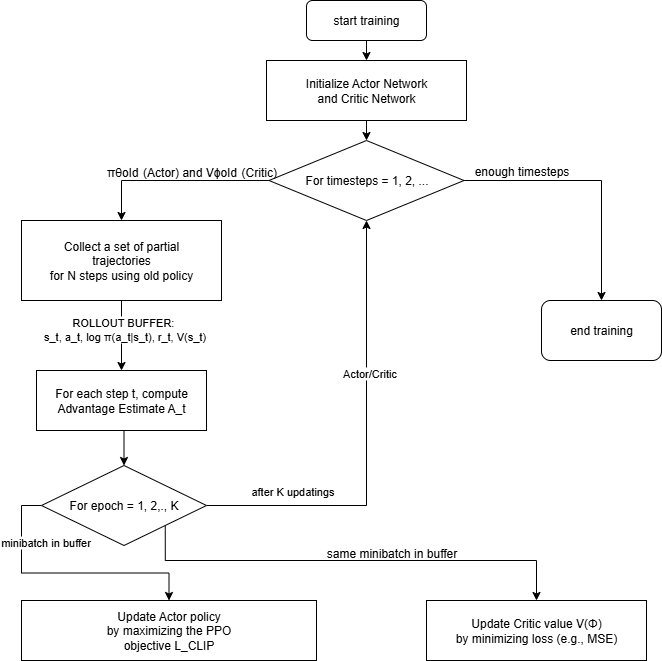
\includegraphics[width=0.7\textwidth]{figures/PPO_training_manual.png}
%     \caption{The PPO training loop data flow. At each iteration, the current policy collects experience into a rollout buffer. Then, advantages are computed, and for several epochs, the actor and critic networks are updated using mini-batches sampled from this buffer.}
%     \label{fig:training_flow}
% \end{figure}

% --- LaTeX Algorithm Code Starts Here ---
\begin{algorithm}[htbp]
\caption{PPO with GAE for Knapsack Problem Training}
\label{alg:ppo}

\SetKwComment{Comment}{\textit{\#}}{}
\SetKwInput{KwPhase}{Phase 1}

% --- Phase 1: Initialization ---
\KwPhase{Initialization}{
    Initialize actor network $\pi_\theta(a|s)$ and critic network $V_\phi(s)$ with shared encoder\;
    Initialize Adam optimizers for parameters $\theta$ and $\phi$\;
    Initialize $N$ parallel `KnapsackEnv` environments\;
}

\BlankLine

\For{each training iteration}{
    
    % --- Phase 2: Rollout (was 2a) ---
    \Comment{--- Phase 2: Rollout / Data Collection ---}
    Initialize an empty Rollout Buffer $\mathcal{D}$\;
    \For{$t = 1 \to \text{n\_steps}$}{
        \For{each parallel environment $i = 1 \to N$}{
            Observe state $s_t^{(i)}$\;
            Sample action $a_t^{(i)} \sim \pi_{\theta_{\text{old}}}( \cdot | s_t^{(i)})$\;
            Compute value $V_\phi(s_t^{(i)})$ and log-probability $\log \pi_{\theta_{\text{old}}}(a_t^{(i)}|s_t^{(i)})$\;
            Execute action $a_t^{(i)}$ to get next state $s_{t+1}^{(i)}$ and reward $r_t^{(i)}$\;
            Let $\tau_t^{(i)} = (s_t^{(i)}, \dots, \log \pi_{\theta_{\text{old}}}(a_t^{(i)}|s_t^{(i)}))$\;
            Store transition $\tau_t^{(i)}$ in $\mathcal{D}$\;
        }
    }
    
    \BlankLine
    % --- Phase 3: Advantage Estimation (was 2b) ---
    \Comment{--- Phase 3: Advantage and Return Estimation ---}
    Compute GAE advantage estimates $\hat{A}_t$ for all transitions in $\mathcal{D}$\;
    Compute returns-to-go $R_t \leftarrow \hat{A}_t + V_\phi(s_t)$ for all transitions in $\mathcal{D}$\;
    
    \BlankLine
    % --- Phase 4: Optimization (was 2c) ---
    \Comment{--- Phase 4: Optimization ---}
    \For{$k = 1 \to \text{n\_epochs}$}{
        \For{each mini-batch of $(s, a, R, \hat{A}, \log \pi_{\text{old}})$ from $\mathcal{D}$}{
            Calculate ratio: $r(\theta) \leftarrow \exp(\log \pi_\theta(a|s) - \log \pi_{\text{old}})$\;
            $L^{\text{CLIP}}(\theta) \leftarrow -\mathbb{E} \left[ \min(r(\theta)\hat{A}, \text{clip}(r(\theta), 1-\epsilon, 1+\epsilon)\hat{A}) \right]$\;
            $L^{\text{VF}}(\phi) \leftarrow \mathbb{E} \left[ (V_\phi(s) - R)^2 \right]$\;
            $S[\pi_\theta] \leftarrow \mathbb{E} \left[ \text{Entropy}(\pi_\theta(s)) \right]$\;
            $L(\theta, \phi) \leftarrow L^{\text{CLIP}}(\theta) + c_1 L^{\text{VF}}(\phi) - c_2 S[\pi_\theta]$\;
            Update parameters $\theta, \phi$ by descending the gradient $\nabla_{\theta,\phi} L(\theta, \phi)$\;
        }
    }
}
\end{algorithm}
% --- LaTeX Algorithm Code Ends Here ---



% \chapter{Experiments and Results}
% !TEX root =  ../Dissertation.tex

\chapter{Experiments and Results}

\input{Chapter5/5.0_Baseline}
% !TEX root = ../Dissertation.tex

\section{Experimental Setup}
\label{sec:experimental_setup}

This section details the experimental framework designed to rigorously evaluate the performance of our proposed Proximal Policy Optimization (PPO) based framework. We outline the objectives, datasets, baseline algorithms, evaluation metrics, and the specific configuration of our model used for testing.

\subsection{Objectives}
The primary objectives of these experiments are twofold:
\begin{enumerate}
    \item To assess the \textbf{generalization performance} of our PPO-based model by training it exclusively on small-scale instances and testing it on a range of larger, unseen problem sizes.
    \item To evaluate the \textbf{computational efficiency} and \textbf{solution quality} of our model in comparison to a comprehensive suite of benchmarks, including classical optimization algorithms, a commercial solver, and alternative neural network architectures.
\end{enumerate}

\subsection{Datasets}
To ensure a robust and fair evaluation, three distinct primary datasets were procedurally generated for training, validation, and testing the generalization performance of the neural models. The parameters for these datasets are summarized in Table~\ref{tab:dataset_specs}.

% --- TABLE HAS BEEN MODIFIED TO FIT PAGE WIDTH ---
\begin{table}[htbp]
    \centering
    \caption{Specification of the Primary Datasets}
    \label{tab:dataset_specs}
    % Font size reduced slightly for a better fit
    \footnotesize
    \begin{tabular}{@{}lccc@{}}
        \toprule
        % The long header is now in a nested tabular to allow it to wrap
        \textbf{Parameter} & \textbf{Training Set} & \textbf{Validation Set} & \begin{tabular}[c]{@{}c@{}}\textbf{Generalization} \\ \textbf{Test Set}\end{tabular} \\
        \midrule
        Item Count Range ($n$) & 5 to 50 & 5 to 50 & \textbf{50 to 200}\\
        Step Size & 5 & 5 & 5  \\
        Instances per Size & 100 & 30 & 50  \\
        \addlinespace
        \textbf{Total Instances} & \textbf{1,000} & \textbf{300} & \textbf{1,300} \\
        \bottomrule
    \end{tabular}
\end{table}

All generated instances across all datasets share a common set of properties.
Item weights ($w_i$) and values ($v_i$) were sampled as integers from a uniform distribution $U[1, 100]$.
There is no explicit correlation between an item's weight and its value.
The knapsack capacity ($C$) for each instance was set relative to the sum of all its item weights ($\sum w_i$), with the capacity ratio randomly sampled from a uniform distribution $U[0.1, 0.9]$.
**This range was chosen to ensure the generated problems are non-trivial; a capacity ratio below 0.1 would result in problems where very few items can be packed, while a ratio approaching 1.0 would allow nearly all items to be included, with both extremes lacking combinatorial difficulty and generality.
** All input features are normalized before being passed to the neural network models, as detailed in Section 4.4.

Furthermore, to empirically analyze the runtime of traditional algorithms on larger problems, a separate \textbf{Scalability Test Set} was generated. This dataset contains instances where the number of items $n$ ranges from 100 to 1000, with a step size of 5 and 10 instances generated per size, for a total of 1,810 instances. The item and capacity properties for this set are identical to those of the primary datasets.
\subsection{Baseline Algorithms}
To provide a thorough evaluation, our proposed PPO framework is benchmarked against three categories of solvers.

\subsubsection{Optimal and Classical Solvers}
These solvers represent traditional, non-learning-based approaches to the Knapsack Problem.
\begin{itemize}
    \item \textbf{Gurobi}: The Gurobi Optimizer is a state-of-the-art commercial solver. It is used in our experiments to provide the certified \textbf{optimal solution (ground-truth)} for each test instance, which is essential for calculating the Mean Relative Error of all other methods.
    \item \textbf{Dynamic Programming (DP)}: We implemented the classic space-optimized 1D DP algorithm. Its theoretical time complexity is $O(nC)$, where $C$ is the knapsack capacity, making it pseudo-polynomial. For instances where capacity scales polynomially with $n$ (as in our test cases), this often results in an empirical runtime that grows polynomially with $n$.
    \item \textbf{Branch and Bound (BnB)}: A standard BnB algorithm was implemented as another exact-method benchmark. While often faster than DP in practice on certain instance types, its worst-case time complexity is exponential.
    \item \textbf{Greedy Heuristic}: A simple greedy algorithm that sorts items by value-to-weight ratio is included as a fast, low-complexity baseline.
\end{itemize}
The high computational cost of classical methods is a core motivation for this research. Figure~\ref{fig:complexity_growth} empirically demonstrates this limitation. On a log-log scale, the runtime of the DP and BnB algorithms grows polynomially, consistent with their theoretical complexity, and becomes prohibitively slow for large $n$. This validates the need for fast, scalable approximation methods like our proposed RL framework.

\begin{figure}[htbp]
    \centering
    \includegraphics[width=0.9\textwidth]{figures/knapsack_loglog.png}
    \caption{Empirical runtime growth of classical algorithms on the Scalability Test Set ($n=100$ to $1000$). The log-log scale clearly shows the polynomial time complexity, with the 1D DP solver's growth aligning with an approximate $O(n^2)$ trend in this experimental setting.}
    \label{fig:complexity_growth}
\end{figure}

\subsubsection{Neural Network Baselines}
To position our work relative to other learning-based approaches, we compare it against two alternative neural architectures.
\begin{itemize}
    \item \textbf{Multi-Layer Perceptron (MLP)}: A standard MLP is trained to directly predict the solution vector. This baseline serves to demonstrate the limitations of simple function approximators that do not explicitly model the combinatorial and sequential nature of the problem.
    \item \textbf{Pointer Network with REINFORCE (Ptr-Net)}: We implemented a Pointer Network based on the seminal work of Bello et al., trained with the REINFORCE algorithm. This model represents an important milestone in RL for combinatorial optimization and serves as a direct benchmark to showcase the superior training stability and performance of our PPO-based approach.
\end{itemize}

\subsection{Proposed Model Configuration}
The model evaluated in this chapter is the final Transformer-PPO architecture detailed in Chapter 4. It utilizes the best-performing configuration identified during our research, which features a shared Transformer encoder and a simple MLP critic head. For complete architectural and hyperparameter details, please refer to Section 4.3 and Section 4.5.

\subsection{Evaluation Metrics}
The performance of all solvers is evaluated based on two primary metrics:
\begin{itemize}
    \item \textbf{Solution Quality}: Measured by the \textbf{Mean Relative Error (MRE)} against the optimal solutions from Gurobi. It is calculated as:
    $$MRE = \frac{1}{N} \sum_{i=1}^{N} \frac{V_{\text{optimal}}^{(i)} - V_{\text{solver}}^{(i)}}{V_{\text{optimal}}^{(i)}}$$
    where $V_{\text{solver}}^{(i)}$ is the value obtained by the evaluated solver for instance $i$, and $N$ is the total number of instances. A lower MRE indicates higher solution quality. An MRE of 0.3 corresponds to 70\% accuracy.
    \item \textbf{Computational Efficiency}: Measured by the \textbf{Average Inference Time} in milliseconds, recorded for each solver to find a solution for a single problem instance.
\end{itemize}

\subsection{Inference Procedure and Decoding Strategy}
\label{sec:inference_procedure}

To generate a complete, sequential solution from the trained static policy network, we employ an autoregressive inference procedure that simulates the agent's interaction with the environment, as detailed in Algorithm~\ref{alg:instance_solver}. This instance-based solver operates in a closed loop: at each timestep $t$, the environment's current state $s_t$ is provided to the PPO model, which then predicts the next item to be selected, $a_t$. Subsequently, the environment updates its internal state to $s_{t+1}$ based on this action (e.g., by reducing the remaining capacity and masking the selected item). This decision-update cycle continues until no further items can be packed, thereby constructing the final solution. This step-by-step process ensures that each decision is conditioned on the most recent and valid state of the knapsack.

For all reported experiments, we utilize a deterministic greedy decoding strategy \texttt{is\_deterministic=True}. This choice serves two primary objectives. First, it consistently evaluates the optimal policy learned by the agent by eliminating stochasticity, which ensures the reproducibility of our results. Second, through preliminary experiments, we determined that introducing stochastic sampling did not yield a significant improvement in solution quality (MRE) but substantially increased computation time. Therefore, to achieve an optimal balance between evaluation efficiency and performance, all results are based on deterministic greedy decoding.

\begin{algorithm}[htbp]
    \caption{Inference Procedure for the Instance-based Solver}
    \label{alg:instance_solver}
    \KwIn{Trained PPO Model $\pi_\theta$, Problem Instance $I$}
    \KwOut{Final solution value $V_{\text{final}}$}
    \BlankLine
    Initialize environment with instance $I$\;
    $s_0 \leftarrow \text{env.reset()}$\;
    $done \leftarrow \text{False}$\;
    \BlankLine
    \While{not $done$}{
        \tcp{Agent makes a decision based on the current state}
        $s_t^{\text{norm}} \leftarrow \text{VecNormalize}(s_t)$\;
        $a_t \leftarrow \pi_\theta(s_t^{\text{norm}})$ using greedy decoding\;
        \BlankLine
        \tcp{Environment transitions to the next state}
        $(s_{t+1}, r_t, done, \text{info}) \leftarrow \text{env.step}(a_t)$\;
        $s_t \leftarrow s_{t+1}$\;
    }
    \BlankLine
    $V_{\text{final}} \leftarrow \text{info.get("total\_value")}$\;
    \Return{$V_{\text{final}}$}\;
\end{algorithm}

\subsection{Hardware and Software Environment}
All experiments were conducted on a consistent hardware platform to ensure fair comparison.
\begin{itemize}
    \item \textbf{CPU}: [12th Gen Intel(R) Core(TM) i5-12500H (16 CPUs), ~2.5GHz]
    \item \textbf{GPU}: [NVIDIA GeForce RTX 2050]
    \item \textbf{Memory}: [16 GB DDR5]
    \item \textbf{Software}: Python 3.11.13, PyTorch 2.7.1, CUDA 12.6, Stable-Baselines3 2.7.0, Gurobi 12.0.2.
\end{itemize}
% !TEX root = ../Dissertation.tex
\section{Results}
% !TEX root = ../Dissertation.tex

\section{Evaluation and Discussion}
\label{sec:discussion}

The results presented in Section 5.2 confirm the effectiveness of our proposed Transformer-PPO framework.
This section provides a deeper analysis of these findings, interpreting the performance differences between the models, discussing the critical role of the underlying architecture and training algorithm, and addressing the limitations and implications of this work.

\subsection{Analysis of Solution Quality (MRE)}
The primary goal of this research was to develop a model capable of generalizing to large-scale problems from training on small ones.
Figure~\ref{fig:mre_vs_size} demonstrates that this objective was successfully met.

Our PPO-based model maintains a low and stable Mean Relative Error (MRE) below 30\% for instances up to $n=200$, showcasing high solution quality.
This success can be attributed to a synergy of three key factors:
\begin{itemize}
    \item \textbf{Algorithmic Superiority}: The PPO algorithm's Actor-Critic structure, which uses Temporal Difference (TD) updates to estimate advantages, provides a low-variance learning signal.
This is substantially more stable than the high-variance Monte Carlo returns used by the baseline Pointer Network's REINFORCE algorithm, which failed to learn an effective policy.
\item \textbf{Architectural Advantage}: The \textbf{Transformer} encoder is crucial for performance.
Its self-attention mechanism processes all items in parallel, capturing the global, combinatorial relationships within the problem instance.
This is a more powerful approach than the sequential processing of an LSTM, which was used in the baseline Pointer Network architecture.
\item \textbf{Framework Robustness}: The use of the \textbf{Stable-Baselines3} framework provides significant benefits, most notably the `VecNormalize` wrapper.
The automatic and adaptive normalization of both observations and rewards during training is a key stabilization technique that was absent in the baseline implementations.
\end{itemize}
In contrast, the baseline MLP model completely failed to generalize, confirming that a simple neural network cannot learn the complex, structured policy required for the Knapsack Problem. It is worth noting, however, that under different problem formulations, such as modeling virtual machine placement as a KP, simpler neural networks have been shown to outperform traditional metaheuristics, highlighting the importance of matching the model architecture to the specific problem representation \cite{abidSolving012023}.

\subsection{Analysis of Computational Efficiency (Inference Time)}
While solution quality is paramount, computational efficiency is critical for practical applications.

\subsubsection{Initial Findings and Architectural Overhead}
As shown in the initial time analysis in Figure~\ref{fig:time_vs_size}, our PPO model is orders of magnitude faster than the optimal Gurobi solver but slower than the neural baselines.
This overhead is expected and stems from two architectural realities:
\begin{itemize}
    \item The \textbf{Transformer} architecture is inherently more computationally intensive than the lightweight LSTM or MLP models.
    \item The Actor-Critic design requires forward passes through both the policy (actor) and value (critic) networks, adding computational cost compared to an actor-only method like REINFORCE.
\end{itemize}

\subsubsection{The Bottleneck: Iterative vs. Batched Evaluation}
A deeper investigation revealed that the primary bottleneck was not the model's architecture, but the evaluation method.
The standard Stable-Baselines3 evaluation loop processes instances iteratively (one by one), which fails to leverage the massive parallel processing power of a GPU.
To demonstrate the model's true inference potential, we developed a custom, proof-of-concept batch solver capable of processing hundreds of instances simultaneously.
The preliminary results of this solver are shown in Figure~\ref{fig:batch_solver_results}.
The time comparison (Figure~\ref{fig:batch_time}) shows that when properly batched, our PPO model's inference time becomes nearly constant and is significantly faster than all other models.
This confirms that the model architecture is highly efficient for parallel execution.
However, as shown in the MRE comparison (Figure~\ref{fig:batch_mre}), the current implementation of this batch solver contains a bug that severely degrades solution quality.
While this component is still under development, these preliminary results strongly indicate that the model's perceived slowness is an artifact of the evaluation script, not a fundamental limitation of the model itself.

\begin{figure}[H]
    \centering
    % Set the width of the subfigure to be larger, which forces a vertical stack.
    % A width around 0.7 to 0.8\textwidth is usually good for vertical layouts.
    \begin{subfigure}[b]{0.7\textwidth}
        \centering
        \includegraphics[width=\textwidth]{figures/batch_errors.png}
        \caption{MRE vs. Problem Size (Batched)}
        \label{fig:batch_mre}
    \end{subfigure}
    
    % A blank line or \vspace adds vertical separation between the figures.
    \vspace{1em} 
    
    \begin{subfigure}[b]{0.7\textwidth}
        \centering
        \includegraphics[width=\textwidth]{figures/batch_time.png}
        \caption{Inference Time vs. Problem Size (Batched)}
        \label{fig:batch_time}
    \end{subfigure}
    
    % This is the main caption for the entire figure.
    \caption{Preliminary results from a custom-built batch evaluation solver. (a) The current implementation shows a degradation in solution quality, which is a work-in-progress.
(b) However, it successfully demonstrates that the PPO model's inference time becomes nearly constant and extremely fast when leveraging batch processing.}
    \label{fig:batch_solver_results}
\end{figure}

\subsection{Analysis of a High-Performance Batched Solver}
\label{sec:analysis_batch_solver}

A primary motivation for employing neural networks in combinatorial optimization is their potential for massive parallelization.
To investigate this, we developed a prototype high-performance solver \texttt{fast\_ppo\_solver} designed to process entire batches of problems simultaneously, aiming for a near-constant inference time, as detailed in Algorithm~\ref{alg:batch_solver}.
The empirical results, presented in Figure~\ref{fig:batch_solver_results}, confirm this solver's speed potential.
As shown in Figure~\ref{fig:batch_time}, the inference time remains constant regardless of problem size, demonstrating the efficiency of leveraging GPU hardware for parallel computation.
However, this gain in speed was accompanied by a severe degradation in solution quality, with the MRE rising dramatically (Figure~\ref{fig:batch_mre}).
This discrepancy between the two solvers provides a critical insight into a common challenge in machine learning deployment: the \textbf{Training-Inference Skew}.

The core of the issue lies in the fundamental difference between the data processing workflows of the two solvers.
The successful instance-based solver (Algorithm~\ref{alg:instance_solver}) operates in a stateful, step-by-step loop.
Crucially, after each item selection, the environment's state (including the \textit{remaining capacity}) is updated, and this entire new state is re-normalized and re-processed by the model's feature extractor.
The model's policy is therefore conditioned on a dynamically updated state representation at every step.
In contrast, the batched solver (Algorithm~\ref{alg:batch_solver}), in its pursuit of efficiency, performs feature extraction and normalization only once on the initial problem state.
Its internal autoregressive decoding loop, while tracking capacity for constraint validation, does not feed this updated state information back into the feature extractor.
Consequently, every decision after the first is based on a stale feature representation derived from the initial state.
The model, which was trained to expect a fully updated and re-normalized state at each step, is thus forced to operate on a data distribution it has never seen, leading to a catastrophic failure of its learned policy.
This finding underscores the critical importance of maintaining strict consistency between the data processing pipelines used during training and inference to ensure a model's performance translates from the research environment to practical application.

\begin{algorithm}[htbp]
    \caption{Inference Procedure for the Batched Solver}
    \label{alg:batch_solver}
    \KwIn{Trained PPO Model $\pi_\theta$, Batch of problem instances $\mathcal{B}$}
    \KwOut{Batch of final solution values $\mathcal{V}$}
    \BlankLine
    \tcp{--- Phase 1: Pre-processing and One-Time Feature Extraction ---}
    $s_0 \leftarrow \text{Construct observation dictionary for batch } \mathcal{B}$\;
    $s_0^{\text{norm}} \leftarrow \text{Manually scale and normalize features in } s_0$\;
    $C \leftarrow \mathrm{FeatureExtractor}(s_0^{\text{norm}})$\;
    \BlankLine
    \tcp{--- Phase 2: Internal Autoregressive Decoding ---}
    $\mathcal{A} \leftarrow \text{empty list}$\;
    Initialize internal capacity tracker and masks\;
    \BlankLine
    \While{decoding is not complete for all instances in batch}{
        \tcp{Decision is based on the initial context C}
        $a_t \leftarrow \mathrm{select\_action}(C, \mathrm{internal\_query\_vector})$\;
        Append $a_t$ to $\mathcal{A}$\;
        \BlankLine
        \tcp{Internal state is updated for constraints only}
        Update internal capacity tracker and masks based on $a_t$\;
        \tcp{Note: The context C is not re-computed}
    }
    \BlankLine
    $\mathcal{V} \leftarrow \text{Post-process sequence } \mathcal{A} \text{ to calculate final values}$\;
    \Return{$\mathcal{V}$}\;
\end{algorithm}

\subsection{Synthesis and Answering Research Questions}
The experimental results, when synthesized, provide comprehensive answers to our core research questions and highlight the trade-offs inherent in deploying complex learned models.

\subsubsection{On Generalization and Solution Quality}
The primary research question concerned the model's ability to generalize from small-scale training instances to larger, unseen problems.
The performance of the instance-based solver (Section~\ref{sec:results}) provides a clear, affirmative answer.
By maintaining a stable, low MRE on instances up to four times the size of its training data, the model demonstrates that it has learned a genuinely scalable and robust policy, successfully avoiding the pitfalls of overfitting to fixed problem dimensions that have limited prior neural approaches.

\subsubsection{On Computational Efficiency and Scalability}
Our second research question addressed the framework's potential for high-speed inference.
The two solver implementations offer complementary insights. The instance-based solver shows favorable scaling relative to exact methods, confirming its practicality.
More significantly, the batched solver experiment (Section~\ref{sec:analysis_batch_solver}) definitively proves the architectural potential for constant-time, $O(1)$ inference.
This result confirms that the Transformer-based model is not just a theoretical construct but is well-suited for high-throughput, real-world applications where decision speed is critical.

\subsubsection{Synthesis: A Robust Framework with Critical Deployment Insights}
In conclusion, the combination of a Transformer architecture with the PPO algorithm is a potent and effective choice for this class of combinatorial optimization problem.
The framework successfully learns a generalizable policy that delivers high-quality solutions.
However, the stark performance contrast between the instance-based and batched solvers reveals a critical finding: the learned policy's effectiveness is deeply coupled to the state representation and processing pipeline used during training.
This discovery of a significant training-inference skew provides a crucial insight for the field, emphasizing that the design of an inference engine is not merely an implementation detail but a core component that must be co-designed with the model and training regime to ensure success.

% \chapter{Conclusion and Future Work}
% !TEX root =  ../Dissertation.tex

\chapter{Conclusion and Future Work}

% !TEX root = ../Dissertation.tex
\section{Conclusions}
% !TEX root = ../Dissertation.tex
\section{Future Work}

\bibliographystyle{abbrv}
\bibliography{bibliography}

% !TEX root = ../Dissertation.tex

\appendix
\chapter{Software Manual}
\label{chap:software_manual}
\addcontentsline{toc}{chapter}{Software Manual}

This appendix provides a comprehensive guide to the software platform developed for this research. The platform is an integrated framework designed to handle the entire research pipeline, including procedural data generation, model training, and comparative evaluation of various solvers.

\section{Code Repository}
The source code is hosted on both GitHub for public access and the University of Birmingham's internal GitLab server for academic version control.

\begin{itemize}
    \item \small\textbf{Public GitHub Repository}: \url{https://github.com/Gavin-spring/ann_kp.git}
    \item \small\textbf{Internal Academic Repository}: \url{https://git.cs.bham.ac.uk/projects-2024-25/gxl386.git}
\end{itemize}

\section{Installation Guide}

\subsection{System Requirements}
\begin{itemize}
    \item \textbf{Operating System}: A Linux-based distribution is highly recommended. The framework leverages Triton to compile and optimize the neural network models, which currently has the most robust support on Linux.
    \item \textbf{Hardware}: An NVIDIA GPU is required for training and evaluation. The codebase is optimized for CUDA and supports mixed-precision training to accelerate performance.
    \item \textbf{NVIDIA CUDA}: CUDA version 12.1 or newer is required.
\end{itemize}

\subsection{Dependencies}
All required Python packages are listed in the \texttt{requirements.txt} file in the root of the repository. Key dependencies include PyTorch, Gymnasium, and Stable-Baselines3.

\subsection{Installation Steps}
A bash script, \texttt{setup\_vlab.sh}, is provided to automate the entire setup process. It is the recommended method for creating a clean and correct environment. Executing this script will perform the following actions:
\begin{enumerate}
    \item Download and install Miniconda, a minimal installer for the Conda package manager.
    \item Create a new Conda virtual environment to isolate project dependencies.
    \item Install all required packages listed in \texttt{requirements.txt} using `pip`.
    \item Install Rclone, a command-line tool for managing files on cloud storage, to facilitate data transfer.
    \item Install ngrok, a reverse proxy tool, to enable remote monitoring of training progress (e.g., via TensorBoard).
\end{enumerate}

\section{File Structure}
The repository is organized into a modular structure to separate concerns and improve maintainability.

\begin{description}
    \item[\texttt{data/}] Contains the datasets for training, validation, and testing. Each problem instance is stored in a `.csv` file.
    \item[\texttt{src/}] Contains the primary source code for the project, including:
        \begin{itemize}
            \item The implementation of the custom Gymnasium environment (\texttt{knapsack\_env.py}).
            \item The source code for all solvers, including classical algorithms and neural network architectures (\texttt{custom\_policy.py}, etc.).
        \end{itemize}
    \item[\texttt{scripts/}] Contains the main entry-point scripts for executing key pipeline stages, such as data generation, model training, and evaluation.
    \item[\texttt{artifacts/}] The default output directory for results generated by the \texttt{train\_model.py} and \texttt{evaluate\_solvers.py} scripts. This includes trained models, logs, and evaluation metrics for the MLP, Pointer Network (REINFORCE), and classical solvers.
    \item[\texttt{artifacts\_sb3/}] A dedicated output directory for all experiments related to the Stable-Baselines3 PPO implementation. Results from \texttt{train\_sb3.py} and \texttt{evaluate\_sb3.py} are stored here.
    \item[\texttt{docs/}] Contains supplementary documentation, including this manual.
    \item[\texttt{config.yaml}] A centralized configuration file for managing all hyperparameters, paths, and experimental settings.
    \item[\texttt{README.md}] The main project README file with an overview and basic instructions.
\end{description}

\section{Running the Code}
The project is packaged using \texttt{setup.py}, which creates convenient command-line entry points for all major scripts. After setting up the environment, the following commands become available system-wide:

\begin{verbatim}
    generate       # For generating new problem instances
    preprocess     # For any data preprocessing steps
    train          # For training the MLP and REINFORCE models
    train-sb3      # For training the final PPO model
    evaluate       # For evaluating all solvers in a unified test
    evaluate-sb3   # For dedicated evaluation of a PPO model
\end{verbatim}

\subsection{Data Generation}
To generate new datasets for the Knapsack Problem:
\begin{enumerate}
    \item Modify the \texttt{data\_gen} section of \texttt{config.yaml} to specify the desired characteristics of the problem instances (e.g., number of items, correlation type).
    \item Ensure the output paths in the `paths` section of \texttt{config.yaml} are set correctly.
    \item Run the command: \texttt{generate}
\end{enumerate}

\subsection{Model Training}
The framework supports training three different neural architectures. All hyperparameters and settings are managed through the \texttt{config.yaml} file.

\subsubsection{Training the Transformer-PPO Model (Primary Contribution)}
This is the primary model presented in this dissertation.
\begin{enumerate}
    \item Navigate to the \texttt{ml.rl.ppo} section in \texttt{config.yaml}.
    \item Adjust the model architecture and training hyperparameters as required. This includes settings for the Transformer encoder (\texttt{embedding\_dim}, \texttt{nhead}, \texttt{num\_layers}), the PPO algorithm (\texttt{n\_steps}, \texttt{gamma}, \texttt{clip\_range}), and the learning rate schedule.
    \item Verify that the \texttt{data\_training} and \texttt{data\_validation} paths are correct.
    \item Execute the training script using the command: \texttt{train-sb3 --name <YourExperimentName>}
\end{enumerate}

\subsubsection{Training the MLP Model}
\begin{enumerate}
    \item Navigate to the \texttt{ml.dnn} section in \texttt{config.yaml}.
    \item Configure the model and training hyperparameters, such as \texttt{total\_epochs}, \texttt{batch\_size}, and \texttt{learning\_rate}.
    \item Verify that the data paths are correct.
    \item Execute the training script using the command: \texttt{train} (ensure \texttt{training\_mode} is set to \texttt{dnn} in the config).
\end{enumerate}

\subsubsection{Training the Pointer Network (REINFORCE / Actor-Critic)}
\begin{enumerate}
    \item Navigate to the \texttt{ml.rl} section in \texttt{config.yaml}.
    \item Select the desired training algorithm by setting \texttt{training\_mode} to either \texttt{"reinforce"} (for EMA baseline) or \texttt{"actor\_critic"} (for critic baseline).
    \item Configure the hyperparameters under the corresponding section (\texttt{reinforce} or \texttt{actor\_critic}).
    \item Verify that the data paths are correct.
    \item Execute the training script using the command: \texttt{train}
\end{enumerate}

\subsection{Model Evaluation}
The framework provides two primary methods for evaluation.

\subsubsection{Dedicated PPO Model Evaluation}
To evaluate a trained PPO model against the Gurobi baseline on a test dataset:
\begin{enumerate}
    \item Execute the command, providing the path to the directory where the trained model and its statistics are saved: \\
    \texttt{evaluate-sb3 --run-dir /path/to/your/artifacts\_sb3/training/ExperimentRun/}
    \item Results, including performance plots and a `.csv` file with detailed metrics, will be saved in a new timestamped directory within \texttt{artifacts\_sb3/evaluation/}.
\end{enumerate}

\subsubsection{Unified Solver Evaluation}
To compare multiple solvers (classical, MLP, Ptr-Net, PPO) simultaneously:
\begin{enumerate}
    \item Open \texttt{src/utils/config\_loader.py} and ensure the solvers you wish to test are active in the \texttt{ALGORITHM\_REGISTRY}.
    \item Execute the \texttt{evaluate} command, providing paths to the trained neural network models: \\
    \texttt{evaluate --dnn-model-path <path> --rl-model-path <path> --ppo-run-dir <path>}
    \item Results are saved in the \texttt{artifacts/results} directory.
\end{enumerate}

\end{document}
